% !TeX encoding = utf8
%
% [ Tiedostossa käytetty merkistö on utf8, vaihtoehtoisesti voisi olla esim.]
% [ ISO 8859-1 eli Latin 1. Ylläoleva rivi ]
% [ tarvitaan, jos käyttää MiKTeX-paketin mukana tulevaa TeXworks-editoria. ]
%
% TIETOTEKNIIKAN KANDIDAATINTUTKIELMA
%
% Yksinkertainen LaTeX2e-mallipohja kandidaatintutkielmalle.
% Käyttää Antti-Juhani Kaijanahon kirjoittamaa gradu3-dokumenttiluokkaa.
%
% Jos kirjoitat pro gradu -tutkielmaa, tee mallipohjaan seuraavat muutokset:
%  - Poista dokumenttiluokasta optio bachelor .
%  - Poista makro \type .
%  - Lisää suuntautumisvaihtoehto makrolla \studyline .
%  - Lisää tieto ohjaajasta makrolla \supervisor .

\documentclass[utf8,bachelor,manualbib]{gradu3}

\usepackage{palatino} % valitaan oletusfonttia hieman tyylikkäämpi fontti

\usepackage{graphicx} % tarvitaan vain, jos halutaan mukaan kuvia
\usepackage{amsmath}  % tarvitaan käytettäessä monimutkaisten matemaattisten kaavojen ja \eqref-kaavaviittauksen yhteydessä
\usepackage{url} % tarvitaan \url-komentoa varten
\usepackage{booktabs}

% Otetaan käyttöön author-date-järjestelmän mukaiset lähdeviittaukset:
\usepackage{natbib}
% Vaihdetaan kirjoittajan nimen ja vuosiluvun väliseksi erottimeksi
% välilyönti (oletuserottimena on pilkku):
%\bibpunct{(}{)}{;}{a}{}{,}


% HUOM! Tämän tulee olla viimeinen \usepackage koko dokumentissa!
\usepackage[bookmarksopen,bookmarksnumbered,linktocpage]{hyperref}

%\addbibresource{viite.bib}% Lähdetietokannan tiedostonimi
%http://www.tex.ac.uk/tex-archive/macros/latex/exptl/biblatex-contrib/biblatex-chicago/latex/biblatex-chicago.sty
%http://www.tex.ac.uk/tex-archive/macros/latex/contrib/etoolbox/etoolbox.sty
%http://mirrors.med.harvard.edu/ctan/macros/latex/contrib/biblatex/latex/biblatex.sty
%http://ctan.mackichan.com/macros/latex/contrib/biblatex/latex/biblatex2.sty
%http://mirror.hmc.edu/ctan/macros/latex/contrib/logreq/logreq.sty
%https://github.com/Martin-Rotter/qt-survival-guide/blob/master/logreq.def

\begin{document}

\title{Keinonäkö- ja parannellun näön järjestelmien käyttöönotto uuden sukupolven ilmailussa}

\translatedtitle{Use of Synthetic and Enhanced Vision Systems in Next Generation Aviation}

%\studyline{}
\avainsanat{TODO}
\keywords{TODO}
\tiivistelma{
Tämä tutkielma käsittelee keinonäkö- ja parannellun näön järjestelmien uuden sukupolven ilmailussa tarjoamia hyötyjä sekä niiden käyttöönotossa ilmeneviä haasteita. Aluksi esitellään näitä järjestelmiä hyödyntäviä näyttölaitteita, sitten lentonäkyvyyden ja tilannetietoisuuden vaikutusta lentoturvallisuuteen, sekä lopuksi ohjaajan pääasiassa kognitiivisista rajoituksista johtuvia haasteita. Näiden tietojen pohjalta pyritään luomaan jonkinlainen kokonaiskuva keinonäkö- ja parannellun näön järjestelmien roolista uuden sukupolven ilmailussa.
}

\abstract{
This bachelor's thesis addresses benefits that synthetic and enhanced vision systems in next generation aviation have to offer, as well as some challenges that might occur in adopting those systems into use.

Aluksi esitellään näitä järjestelmiä hyödyntäviä näyttölaitteita, sitten lentonäkyvyyden ja tilannetietoisuuden vaikutusta lentoturvallisuuteen, sekä lopuksi ohjaajan pääasiassa kognitiivisista rajoituksista johtuvia haasteita. Näiden tietojen pohjalta pyritään luomaan jonkinlainen kokonaiskuva keinonäkö- ja parannellun näön järjestelmien roolista uuden sukupolven ilmailussa.}

\author{Matias Laitinen}
\contactinformation{\texttt{matias.laitinen@gmail.com}}
% jos useita tekijöitä, anna useampi \author-komento

\supervisor{Vesa Lappalainen}
\supervisor{Kirsi Valjus}
% jos useita ohjaajia, anna useampi \supervisor-komento
%\type{bachelor} % tämän makron oletus on "pro gradu -tutkielma" ja bachelor-optiolla kandidaatintutkielma

\maketitle
  
\mainmatter

\chapter{Johdanto}

Lentoturvallisuusasiat nousevat esille medioissa, kun ilmailussa tapahtuu lento-onnettomuuksia tai vaaratilanteita, sillä niissä on osallisena enemmän ihmisiä kuin esimerkiksi tieliikenneonnettomuuksissa. Nämä onnettomuudet aiheutuvat usein inhimillisistä virheistä huonon näkyvyyden olosuhteissa, kun tilannetietoisuuden (Situational Awareness, SA) menetyksen riski on suuri \citep{kimkaber2014, prinzelym2013, schnellym2004, vygolov2013}.

FSF:n (Flight Safety Foundation) mukaan miltei 60\% kaupalliseen lentotoimintaan liittyvistä maahansyöksyonnettomuuksista on tapahtunut lähestymisen tai laskeutumisen aikana \cite{schnellym2004, kimkaber2014}. Ohjattavissa olevan ilma-aluksen tahaton törmäys maahan, veteen tai esteeseen (Controller Flight Into Terrain, CFIT) on vallitseva onnettomuustyyppi ja vastuussa yli puolesta kaupallisen ilmailun onnettomuuksista \citep{etherington2000}. CFIT-onnettomuudet liittyvät yleensä paikka- tai asentotiedon menetykseen lähestymis- ja laskuvaiheessa \cite{schnellym2004}.

Tämän tutkielman tavoitteena on selvittää kirjallisuuskatsauksen keinoin, millä eri tavoin keinonäköjärjestelmiä (Synthetic Vision System, SVS) ja parannellun näön järjestelmiä (Enhanced Vision System, EVS) käyttämällä on mahdollista parantaa lentäjän tilannetietoisuutta ja mahdollistaa turvallinen ja tehokas lentotoiminta jopa huonon näkyvyyden olosuhteissa. Tällaisia järjestelmiä on ollut sotilasilmailun käytössä jo pitkän aikaa, mutta siviili-ilmailussa niitä hyödynnetään vielä melko vähän. Kartoittamalla tällaisten järjestelmien käytettävyyttä ja soveltuvuutta eri tilanteisiin pyritään tekemään johtopäätöksiä niiden turvallisesta käyttöönotosta uuden sukupolven ilmailussa.

Keinonäkö- ja parannellun näön järjestelmien toiminnan kannalta on oleellista, miten järjestelmien tarjoamaa tietoa voidaan esittää ohjaajalle \citep{kimkaber2014}. Toisessa luvussa perehdytään ohjaamoissa käytössä oleviin näyttölaitteisiin. 

\chapter{Näyttölaitteet}

\section{Lasiohjaamo}

Ns. lasiohjaamossa ainakin päälentomittarit on korvattu suurehkolla päänäytöllä (Primary Flight Display, PFD), jossa voidaan esittää mittaritieto selkeästi yhdellä näytöllä keinohorisonttia korostaen. PFD:tä tai muita ohjainpaneeliin sijoitettuja näyttöjä kutsutaan sijaintinsa vuoksi pää alhaalla -näytöiksi (Head-down Display, HDD) SVS/EVS-tietoa voidaan esittää kootusti tällaisilla näytöillä ja ohjaaja voi joissakin tapauksissa itse valita, mitä näytöillä näkyy.

\section{Heijastysnäytöt}

Tietoa voidaan esittää myös heijastusnäyttöjen (Head-up Display, HUD) avulla. Heijastusnäytössä haluttu informaatio ja symbolit heijastetaan läpinäkyvälle näytölle ohjaajan eteen. Tällöin on mahdollista nähdä yhtä aikaa näytöllä oleva mittaritieto sekä ulkona koneen edessä oleva näkymä, mikä mahdollistaa vähemmän aikaa käytettävän mittaritaulun tarkkailuun ja ympäristön seuraaminen on helpompaa \citep{crawfordneal2006}. Verversin ja Wickensin \citeyearpar{ververswickens1998} mukaan tähän vaikuttavat myös HUD:n symboleita selkeyttävät paremmat kontrastierot, HDD:n visuaalisen tiedon mukauttamisen tarpeesta aiheutuva viive.

Tiedon näyttötapa tulisi valita siten, ettei se vie liikaa ohjaajan huomiota pois ulkona olevasta näkymästä. Huomiokyvyn kaventumisesta kerrotaan tarkemmin tämän tutkielman neljännessä luvussa.

Ensimmäiset HUD:t olivat käytössä 1950-luvulla ja niitä käytettiin pääasiallisesti tähtäiminä, eikä lentomittaristona \citep{crawfordneal2006}. Ensimmäistä kertaa heijastusnäyttö oli käytössä koneen lentomittaritiedon näyttämiseen tarkoitettuna välineenä Hawker Siddeley Buccaneer -koneessa vuonna 1960 \citep{weintraubensing1992}. Tämä näyttö koostui keinohorisontista sekä lentokoneen asentoa esittävästä symbolista. Korkeus ja nopeus näytettiin digitaalisesti ja ohjaintietokone tuotti karkeaa opastustietoa. Vielä nykyäänkin heijastusnäytöissä käytetään samankaltaisia symboleja (kuvio \ref{F:HUD}). Näytöstä on hyötyä visuaalisena apuna varsinkin kahdessa päätehtävässä: näkölähestymisessä sekä siirryttäessä mittarilento-olosuhteista visuaaliseen laskeutumiseen. \citep{crawfordneal2006}

HUD:t ovat tulossa käyttöön myös yleisilmailun käyttöön osaltaan sotilas- ja siviili-ilmailussa havaittujen etujen ansiosta \citep{ververswickens1998}. Crawford ja Neal \citeyearpar{crawfordneal2006} toteavat, ettei sotilaspuolen tutkimustuloksia voida helposti soveltaa sellaisenaan kaupalliselle sektorille erilaisen varustuksen ja lentotilanteiden vuoksi.

Verrattuna saman informaation näyttämiseen näkökentän alapuolella sijaitsevassa perinteisessä mittaritaulussa tai HDD-näytöillä, voidaan heijastysnäyttöä käyttäessä tyypillisesti saavuttaa parempi suorituskyky seuraavilla alueilla:

\begin{itemize}
\item Vähemmän aikaa katse mittaritaulussa (head-down -time) kriittisissä lennon vaiheissa ja vähemmän tarvetta tarkentaa katsetta läheltä mittareista kauas ulkomaailmaan \citep{maywickens1995}
\item Parempi lentoreitin säilyttäminen \citep{fischerym1980, lauberym1982, wickenslong1995}
\item Parempi tietoisuus ulkomailmasta ja odotettavissa olevien tapahtumien tai varoitusten havaitseminen ulkona tai näytöllä \citep{faddenym2000, fischer1979, larishwickens1991, maywickens1995, wickenslong1995}
\item Tarkemmat laskeutumiset \citep{naish1964}
\item Paremmat nousu- ja laskeutumisminimit joillakin lentokentillä ja ilma-alustyypeillä \citep{crawfordneal2006}
\item Parempi laatu mittaritiedon näyttämisessä \citep{maywickens1995}
\end{itemize}

Tutkielman seuraavassa luvussa käsitellään lentotoiminnassa esiintyviä haasteita sekä keinonäkö- ja parannellun näön järjestelmien niihin mahdollisesti tuomia helpotuksia.

\begin{figure}[t]
\centering
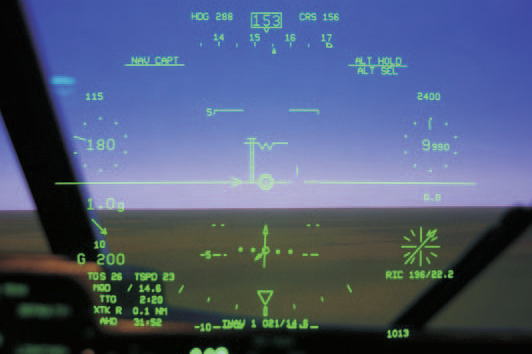
\includegraphics[width=12cm]{HUD.png}
\caption{\itshape Rockwell Collins Flight Dynamics -heijastusnäyttö \citep{crawfordneal2006}.}
\label{F:HUD}
\end{figure}

\chapter{Lento-olosuhteet ja tilannetietoisuus}

\section{Näkyvyys}

Näkyvyys on lentokoneen ohjaajalle tärkeää lennettäessä lähellä maata, ja etenkin lähestymisen ja laskeutumisen aikana. Sen vuoksi huonot näkyvyysolosuhteet aiheuttavat suuria rajoitteita lentotoiminnalle \citep{mollersachs1994, prinzelym2013}. Ohjaajan lentonäkyvyyteen vaikuttavat monet meteorologiset olosuhteet, kuten pimeys, pöly, sumu ja sade \citep{wickensalexander2009}. Erityisesti sumuisissa olosuhteissa näkyvyys voi huonontua voimakkaasti ja ulkomaailman yksityiskohtia on miltei mahdotonta erottaa \citep{beiergemperlein2004}.

Kaikilla lentokentillä toimittaessa ovat voimassa tietyt näkyvyysrajoitukset. Kentillä, joilla on käytössä esimerkiksi ILS:n (Instrument Landing System) kaltaisia lähestymisjärjestelmiä, on olemassa tietty minimi, johon päästäessä tulee olla mahdollista jatkaa lähestymistä visuaalisesti. Eniten rajoitukset vaikuttavat kentillä, joilla ei tällaisia järjestelmiä ole. Myös silloin, kun lähestyvällä koneella on käytössään nykyaikaiset mittari- ja navigointilaitteet. \cite{mollersachs1994}.

Jo ilmailun alkuajoista asti on ilmailuteollisuus kehittänyt laitteita, joilla voittaa näitä huonon näkyvyyden rajoituksia. Tällaisia voivat olla esimerkiksi lentoasentojärjestelmät, navigointilaitteet, mittarilähestymislaitteet (Instrument Landing System, ILS), liikkuva kartta -laitteet (Moving Maps) sekä maastoesteistä varoittavat järjestelmät (EGPWS, Enhanced Ground Proximity Warning System; Terrain Awareness and Warning Systems, TAWS). Näissä voidaan kuitenkin havaita se ongelma, että kaikki nykyaikaisetkin informaation esittämiseen tarkoitetut järjestelmät vaativat ohjaajilta jatkuvaa tiedonhakua ja -käsittelyä pysyäkseen selvillä ilma-aluksensa tulevista liikkeistä huonon näkyvyyden olosuhteissa \citep {prinzelym2004}.

Parannellun näön järjestelmillä (Enhanced Vision System, EVS / Enhanced Flight Vision System, EFVS) käsitetään elektronisen apuvälineen, kuten lämpökameran (Forward-Looking Infrared, FLIR) tai millimetritutkan (Millimeter Wave Radar, MMWR) avulla näytettyä kuvaa ulkomaailmasta \citep{baileyym2007}. Möller ja Sachs \citeyearpar{mollersachs1994} selventävät optisten järjestelmien olevan passiivisia laitteita, joilla voidaan muodostaa ympäristökuva ilman etäisyystietoa. Sitä vastoin esimerkiksi tutkalla saadaan aktiivisesti etäisyystietoa ympäristöstä, mutta tavallisen näköistä kuvaa on vaikea muodostaa.

Kuten Crawford ja Neal \citeyearpar{crawfordneal2006} mainitsevat, voidaan EV-järjestelmiä käyttää yhdessä sekä heijastusnäyttöjen että ohjauspaneelin näyttöjen kanssa, tarjoten lentäjälle lämpökamerakuvaa maastosta ja liikenteestä myös heikoissa valaistus- ja sääolosuhteissa. Prinzel ym. \citeyearpar{prinzelym2013} toteavat huonon näkyvyyden aiheuttamien toiminnan hidastumisten ja viivästysten maatoiminnassa olevan kasvavasti vaikuttamassa myös ilmatilankäytön viiveisiin. Huonon näkyvyyden olosuhteissa ohjaajien ja ajoneuvonkuljettajien tulee säilyttää tilannetietoisuutensa varmistaakseen, että maatoiminta on turvallista ja tehokasta. FAA:n mukaan \citeyearpar{gerold2001} Lennon vaarallisin vaihe onkin juuri maassa rullaaminen. Hooeyn \& Foylen \citeyearpar{hooey2007} tutkimuksen mukaan 17\%:ssa yö- tai huonon näkyvyyden olosuhteissa tapahtuneista rullauskokeista tuli esille navigointivirheitä, jotka saatiin korjattua liikkuvien lentokenttäkarttojen (Airport Moving Map, AMM) avulla. Liikkuvat kartat parantaisivat huomattavasti ohjaajan tilannetietoisuutta, toteavat Möller ja Sachs \citeyearpar{mollersachs1994}.

\section{Tilannetietoisuus}

Hyvän tilannetietoisuuden ylläpitäminen on erittäin olennaista turvallisen lennon kannalta. Hyvä näkyvyys luonnollisesti edesauttaa tilannetietoisuuden säilyttämistä. Schnell ym. \citeyearpar{schnellym2004} toteavat tilannetietoisuuden olevan menetetty, mikäli ohjaamomomiehistö ei osaa vastata seuraaviin kysymyksiin:

\begin{itemize}
\item Missä ollaan?
\item Minne ollaan menossa?
\item Mitä tehdä, kun päästään sinne?
\end{itemize}

Lennettessä mittarilähestymisiä haastavissa olosuhteissa on tärkeintä tietää oman tilankäytön vaatimukset ja maaston niille asettamat rajoitukset. Lisäksi Schnell ym. \citeyearpar{schnellym2004} mainitsevat tilannetietoisuuden liittyvän tilankäytön lisäksi myös ajankäyttöön, sillä ohjaamomiehistön tulisi olla jatkuvasti selvillä siitä, mitä tehtäviä on suoritettava missäkin vaiheessa lentoa. 

Varsinkin suurta tarkkuutta vaativissa lähestymisissä voisi keinonäkö- ja parannellun näön järjestelmien käyttäminen mahdollistaa \citep{schnellym2004}:

\begin{itemize}
\item Pienemmän erotuksen, lähestyttäessä vierekkäisille kiitoteille
\item Turvallisemman estevarakorkeuden säilyttämisen, käytettäessä kaartolähestymisiä haastavilla kentillä, joille suorat lähestymiset eivät onnistu
\end{itemize}

FAA:n vuoden 2010 turvallisuusselvityksen mukaan 52 928 316 maatoimintaan liittyvän tapahtuman aikana tapahtui 951 kiitotiepoikkeamaa (Runway Incursion), joista 12 oli vakavia. Vaikka tämä luku on suhteessa pieni, kiitotiepoikkeamalla voi olla tuhoisat seuraukset. Suurimpana syynä näissä tapauksissa oli ohjaajan inhimillinen erehdys (63 \%). Tilannetietoisuutta parantamalla voitaisiin siis saada merkittävästi vähennettyä kiitotiepoikkeamien määrää. \citep{prinzelym2013}.

Maatoiminnassa lennonjohdon, koneiden ohjaajien sekä ajoneuvonkuljettajien tilannetietoisuutta pyritään pitämään yllä tarjoamalla visuaalisia merkkejä omasta sijainnista, kulkureiteistä ja tilasta kiito- ja rullausteillä, odotuspaikoilla ja asematasoilla. Tämä hoidetaan valojen, merkintöjen ja opasteiden avulla. Tällaisia järjestelmiä kutsutaan yhteisnimellä Surface Movement Guidance and Control System (SMGCS). \citep{prinzelym2013}.

Maatoiminnan tilannetietoa ylläpitäviä järjestelmiä voitaisiin myös käyttää ohjaamoissa. Tällaisista järjestelmistä voisi Prinzelin ym. \citeyearpar{prinzelym2013} mukaan olla hyötyä, varsinkin miehistön näkyvyyden parantamisessa keinotekoisesti sekä paikka- ja reitti-,  mahdollisesti myös liikenne- ja estetiedon parantamisessa erilaisten karttajärjestelmien avulla. Etenkin yöllä, tai savun tai pölyn haitatessa näkyvyyttä, EV-järjestelmät voivat auttaa ohjaajia toimimaan turvallisemmin maassa \citep{prinzelym2013}. Käyttämällä infrapunakameroita, jopa tiheän sumun olosuhteissa havaittaisiin paremmin esteitä, kuten henkilöstöä, ajoneuvoja ja laitteistoja \citep{beiergemperlein2004}.

Pelkkä EVS-järjestelmien käyttö ilman karttaa ei merkittävästi paranna toimintaa maassa. Myös ohjaajat arvioivat AMM -karttojen helpottavan olennaisesti maatoimintaa. Parannellun näön järjestelmiä ja lentokenttäkarttoja yhdistävä E-SMGCS (kuvio \ref{F:E-SMGCS}) voisi parantaa tilannetietoisuutta olennaisesti. Toiminta olisi näin mahdollista entistä huonomman näkyvyyden olosuhteissa kentillä, joilla on vain vähän tai ei lainkaan rullausta avustavia järjestelmiä käytössä. \citep{prinzelym2013}.

\begin{figure}
\centering
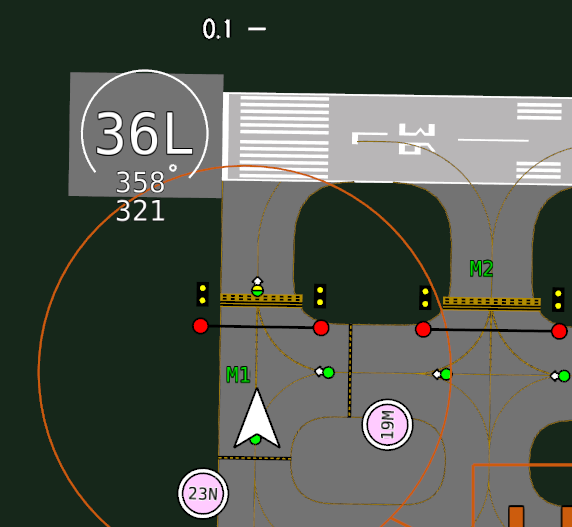
\includegraphics[width=12cm]{E-SMGCS.png}
\caption{\itshape E-SMGCS \citep{prinzelym2013}.}
\label{F:E-SMGCS}
\end{figure}

Tilannetietoisuuden kadotessa hetkellisesti lennolla, voidaan joutua epätavalliseen lentotilaan. Tällöin on olennaista, kuinka nopeasti tilannetietoisuus saadaan palautettua ja virheellinen lentoasento tehokkaasti oikaistua. Käytettäessä perinteisiä mittareita tai ohjainpaneelissa sijaitsevaa näyttölaitetta, voidaan helposti värien avulla kertoa ohjaajalle, missä päin maa ja taivas sijaitsevat. Sen sijaan ainakin nykyiset monokromaattiset heijastusnäytöt vaikeuttavat oikaisua, kun lennetään mittarilento-olosuhteissa ja joudutaan yllättäen epätavalliseen lentotilaan \citep{crawfordneal2006}.

Keinonäköjärjestelmillä (Synthetic Vision System, SVS / Synthetic Vision Information System, SVIS) luodaan tietokoneella keinotekoinen ympäristökuva \citep{baileyym2007}. Käsitteellä voidaan tarkoittaa myös erityisesti NASA:n Rockwell Collinsin kanssa kehittämää samannimistä järjestelmää, SVS \citep{crawfordneal2006}. NASA:n ilmailuturvallisuusohjelman osana SVS:n tarkoituksena on eliminoida huono näkyvyys lento-onnettomuuksien aiheuttajana sekä parantaa yleis- liike- ja kaupallisen ilmailun operationaalisia valmiuksia \citeyearpar{prinzelym2004}.

Kuva luodaan yhdistäen lentoasento- ja tarkkuusnavigointijärjestelmiltä sekä maasto- ja estetietokannoista saatua lennon kannalta tärkeää tietoa. \cite{schnellym2004} toteavat SVIS -järjestelmien olevan uuden sukupolven ohjaamojärjestelmä, joka tulee olemaan tärkeässä osassa tulevaisuuden kaupallisten lentokoneiden ohjaamoissa. Crawford ja Neal kuitenkin \citeyearpar{crawfordneal2006} huomauttavat, että tieto ei välttämättä ole aina täysin ajan tasalla, koska se on peräisin tietokannasta. He mainitsevat myös tiedonkäsittelystä aiheutuvan viiveen voivan aiheuttaa hämmennystä, mikäli näkyvyyden palautuessa visuaalinen näkymä ei olekaan yhtenevä järjestelmän esittämän tiedon kanssa.

Suunnitellessa uusia ohjaamoita voidaan ottaa luonnollisesti huomioon SV-näyttöjen tarpeet (forward fit), mutta oman haasteensa asettaa se, miten käytännölliset ja toimivat näyttölaitteet voidaan asentaa vanhempiin ohjaamoihin, tai ohjaamoihin, joissa tilaa on rajallisesti (retro fit). Eräs ratkaisu tilankäyttöön olisi näyttää SVS heijastusnäytöllä, jolloin voitaisiin keskittyä siihen, kuinka parhaiten esittää keinotekoista kuvaa maastosta sen rajoitettujen grafiikkaominaisuuksien vuoksi. Toinen tapa olisi poistaa perinteiset mittarit ja asentaa tilalle keinonäkönäytöt, jolloin puolestaan jäisi selvitettäväksi, millaiset näyttöesitykset toimivat parhaiten miehistön näkökulmasta. Esimerkiksi yleisten ja fotorealististen tekstuurien maastotekstuurien käytössä ei olla huomattu suorituskykyeroja ohjaajien välillä, mutta ohjaajat tuntuivat pitävän tuloksista huolimatta fotorealistisia tekstuureja parempana vaihtoehtona. NASA:n ilmailuturvallisuusohjelma onkin tutkimassa keinonäkökonseptia, joka yhdistää yleisten ja fotorealististen tekstuurien tilannetietoisuutta parantavat puolet. \citep{prinzelym2004}.

Newman \citeyearpar{newman2000} on listannut heijastusnäyttöjen ominaisuuksia, jotka saattavat vaikeuttaa oikaisua epätavallisista lentotiloista:

\begin{itemize}
\item Merkistön sekavuus (Clutter)
\item Näytön kehykset (Framing)
\item Silmän luontaista tarkentumista häiritsevät tekijät (Accommodation traps)
\item Ylösalaiset symbolit
\item Digitaalisen tiedon esittämisen haasteet
\item Todellisen kokoiset pituuskallistusmerkinnät
\item Näytön käyttäytyminen ohitettaessa suoraan ylös (zenith) tai alas (nadir) -merkinnät
\item Nopeusvektorin hallinnan haasteet
\end{itemize} 

Digitaalisessa muodossa olevan tiedon hahmottaminen nopeasti voi olla hankalaa, mutta analogiset nauhat ja osoittimet voivat lisätä heijastusnäytön sekavuutta \citeyearpar{zuschlag2003}. Todellisen kokoiset pituuskallistusmerkinnät voivat nopeasti edetessään olla myös vaikeita hahmottaa. Newmanin \citeyearpar{newman1995} mukaan tällaisissa tilanteissa pituuskallistusmerkintöjen tiivistäminen hidastaisi niiden liikettä ja ohjaaja voisi paremmin tunnistaa epätavalliseen lentotilaan joutumisen. Mikäli heijastusnäytön nopeusvektorisymbolia käytetään hallitsevana havaintotekijänä voidaan joutua tilaan, jossa todellinen kohtauskulma on ylempänä kuin lentosuunta ja tällöin on virheellistä vetää sauvasta, vaikka nopeusvektori onkin matalalla \citep{crawfordneal2006}. FAA on ohjeistanut näyttöjen suunnittelijoita ottamaan huomioon, että mikäli heijastusnäytöllä käytetään erityistä merkistöä ohjeistamaan oikaisussa vaadittavia ohjainliikkeitä, tulisi käyttää sellaisia symboleja, jotka eivät sekoitu tavanomaisesti näkyvissä oleviin indikaattoreihin \citep{crawfordneal2006}.

Newman \citeyearpar{newman2000} mainitsee heijastusnäyttöjen käyttämisessä saavutettavat hyödyt ylittävät niiden mahdolliset haittavaikutukset. Monista nykyaikaisista varoitujärjestelmistä poiketen SVS-järjestelmät voisivat osaltaan jo ennaltaehkäistä vaarallisiin tilanteisiin joutumista, sen sijaan että toimivat vasta tilanteen ilmetessä. \citep{schnellym2004}. Bennet ja Flach \citeyearpar{bennetflach1994} toteavat tiedon näyttämisen ohjaamoissa dynaamisten ja graafisten esitysten avulla johtavan ihmiskeskeisempään malliin, jossa jatkuva tiedonsaanti näyttäisi luonnollisen kaltaiset rajat turvalliselle toiminnalle. Tällöin korostuisi ihmisen joustavuus käyttää luonnollista ja koodattua informaatiota parhaiten hyväkseen.

Luonnollisella informaatiolla käsitetään tietoa, jota saadaan samalla tavoin kuin näkölento-olosuhteissa katsomalla ulos ohjaamosta. Koodattu informaatio sen sijaan vaatii ohjaajalta erikseen sen todellisen arvon ymmärtämistä. Luonnollista informaatiota voi olla esimerkiksi korkeuden silmämääräinen arviointi ja koodattua informaatiota korkeusmittarin näyttämä \citep{prinzelym2004}. SVS-järjestelmien avulla voidaan esittää tällaista luonnollisen kaltaista ja intuitiivista informaatiota, jota on helppo käsitellä \citep{wickensandre1990}.

SVS-teknologia mahdollistaa rajoitetusta näkyvyydestä aiheutuvien ongelmien ratkaisemisen visuaalisesti, tehden lentotoiminnasta säästä riippumatta samanlaista kuin näkölento-olosuhteissa ja parantaen ohjaajien tilannetietoisuutta \citep{prinzelym2004}. Koska rajoittunut näkyvyys on suurimpana tekijänä monissa kohtalokkaissa lento-onnettomuuksissa \citep{boeing1996}, voisi SVS:n käytöllä olla merkittävä vaikutus turvallisuuteen. Jo pelkät lentoturvallisuuden hyödyt, joita SVS mahdollistaa, ovat tarpeeksi aiheen tutkimiselle, mutta koska tällaisen järjestelmän toteutus on hyvin kallista, on löydettävä myös operationaalisia ja taloudellisia hyötyjä \citep{prinzelym2004}.

Tällaisia hyötyjä NASA \citeyearpar{williamsym2001} arvioi voitavan saavuttaa kasvavan lentoliikenteen myötä seuraavien etujen kautta:

\begin{itemize}
\item Pienempi ajankäytön tarve kiitotiellä huonon näkyvyyden olosuhteissa
\item Pienemmät lähtö- ja saapumisminimit
\item Helpommin sallittavat erilaiset lähestymistavat, etenkin rinnakkaisille kiitoteille
\item Pienemmät porrastukset saapuvien ilma-alusten välillä
\item Toisistaan riippumattoman toiminnan mahdollistaminen rinnakkaisilla, lähekkäin sijaitsevilla kiitoteillä
\end{itemize} 

Schnellin ym. \citeyearpar{schnellym2004} mukaan SVIS-järjestelmät antavat ohjaajille tehtäväkohtaista tietoa ja opastusta, jota tarvitaan lennettäessä monimutkaisia, kaartuvia lähestymispolkuja. Lisäksi he toteavat nykyisen ilmatilan olevan varsinkin joillain lähestymisalueilla kapasiteettinsa rajoilla. Jo pieniki muutos säätilassa tai laitteisto-ongelmat lentokentällä voivat aiheuttaa liikenteen ruuhkautumisen. SVIS-järjestelmistä kaavaillaan mahdollista ratkaisua tähän.

\cite{baileyym2007} väittävät SVS-järjestelmillä saatavan huomattavia parannuksia maastoestetietouteen ja voitavan vähentää CFIT-onnettomuuksien riskiä nykyiseen ohjaamoissa käytettävään teknologiaan verrattuna. Tästä samaa mieltä ovat myös \cite{schnellym2004} todetessaan, että SVIS voisi olla avainteknologia CFIT-onnettomuuksien vähentämisessä.

Tutkijat selvittävät EVS- ja SVS-järjestelmien yhdistämismahdollisuuksia (Enhanced Synthetic Vision System). Tällainen järjestelmä voisi antaa ohjaajalle liikennetietoa samalla tavoin kuin lennettäessä selkeässä säässä päivänvalossa (kuvio \ref{F:ESVS}). Esitettäessä paljon tietoa eri järjestelmistä samalla näytöllä on otettava huomioon inhimilliset tekijät, lentäjän suorituskyky, mahdolliset ongelmat ja turvallisuusnäkökohdat. \citep{crawfordneal2006}

Nordwallin \citeyearpar{nordwall1993} mukaan heijastusnäytön ja lämpökameran yhdistelmällä saavutetaan sumussa huomattavasti parempi kuva ynpäristöstä, kuin mitä paljaalla silmällä voitaisiin. Beierin ja Gemperleinin \citeyearpar{beiergemperlein2004} tutkimuksen perusteella aivan tiheässä sumussa, jossa näkyvyydet ovat 300 m tai vähemmän, ei edes lämpökameroita käyttämällä kuitenkaan saada parannusta näkyvyyteen. Myös Crawford ja Neal \citeyearpar{crawfordneal2006} toteavat kovan sumun, sateen tai pölyn heikentävän lämpökameralla saavutettavia etuja. Tällaisissa tapauksissa lähestymisessä tarvittaisiin esimerkiksi tutkajärjestelmä luomaan ympäristökuvaa.

\begin{figure}[t]
\centering
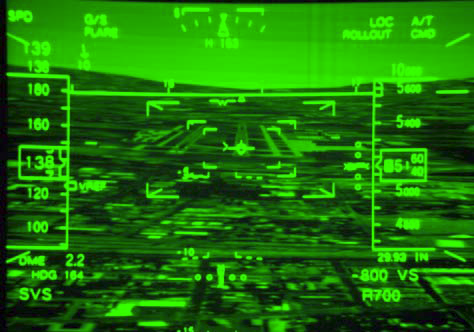
\includegraphics[width=12cm]{HUD_Fused.png}
\caption{\itshape Yhdistetty ESVS heijastusnäytöllä \citep{baileyym2007}.}
\label{F:ESVS}
\end{figure}

Baileyn ym.\citeyearpar{baileyym2007} mukaan näiden teknologioiden optimaalisin yhdistelmä olisi näyttää ohjaamomiehistölle suoraan SVS-järjestelmän informaatiota, mutta EVS-järjestelmän kuvanprosessointi toimisi taustalla, suorittaen navigaatiovirheiden korjausta, tietokannan eheyden valvontaa sekä reaaliaikaista esteentunnistusta.

Schnell ym. \citeyearpar{schnellym2004} lisäävät, että SVIS:n käyttö yhdessä GPS-navigointijärjestelmien kanssa voisi mahdollistaa uusia jatkuvan liu'un kaartolähestymismenetelmiä, jotka olisivat nykyisiä suoria ja portaittaisia lähestymisiä tehokkaampia. Tällaisia lähestymismenetelmiä miehistön on vaikeaa suorittaa perinteisillä lentonäyttöjärjestelmillä. Etenkin ajallisesti kaartolähestymisiä on haastavaa käsittää verbaalisesti tai paperilla. SVIS helpottaisi asiaa ilmassa sijaitsevalla, keinotekoisella, kolmiuloitteisella tunnelilla, jota on helppo seurata \citep{barrowspowell1999}.

\section{NGATS ja EVO}

NASA on kehittämässä ns. uuden sukupolven ilmakuljetusjärjestelmä (Next Generation Air Transport System, NGATS), jossa keskeisenä on uutta avioniikkateknologiaa hyödyntävä EVO-konsepti (Equivalent Visual Operations) \citep{baileyym2007}. Siinä keinonäkö- ja näönparannusjärjestelmiä käyttäen saataisiin tarpeeksi tietoa ympäristöstä, jotta voitaisiin ulkoisista näkyvyysolosuhteista riippumatta toimia aina näkölentosääntöjen mukaisesti. Tällainen menettely mahdollistaisi näkölento-olosuhteiden mukaisen operatiivisen toimintatahdin huonommalla säällä ja parantaisi turvallisuutta ennestään myös hyvän näkyvyyden olosuhteissa \citep{prinzelym2013}.

\chapter{Lentotietojärjestelmien käytön haasteita}

\section{Huomiokyvyn kaventuminen (Attentional tunneling)}

Ohjaajan on tyypilliseti helpompi havaita ulkona tapahtuvia asioita ja hallita lentorataansa, kun katsetta ei tarvitse jatkuvasti siirrellä ulkonäkymän ja mittaritaulun välillä \citep{crawfordneal2006, ververswickens1998}. Useat tutkimukset \citep{fischerym1980, kimkaber2014, weintraubensing1992, wickenslong1995, wickensalexander2009} kuitenkin osoittavat, että heijastusnäytön symbolit voivat kiinnittää liikaa ohjaajan huomiota puoleensa ja heikentää hänen kykyään havainnoida ennalta odottamattomia ympäristön tapahtumia. Samankaltaisesta ilmiöstä on kyse, kun esimerkiksi puhutaan puhelimeen autolla ajaessa, mikä voi johtaa huomion keskittymiseen keskusteluun ajamisen sijaan \citep{horreywickens2006, strayerdrews2007, strayerym2001}. Wickens ja Alexander \citeyearpar{wickensalexander2009} toteavat, että näkökentän sisälläkään olevat objektit eivät automaattisesti herätä tarpeeksi huomiota ja määrittelevät huomiokyvyn kaventumisen (attentional tunneling): \emph{"The allocation of attention to a particular channel of information, diagnostic hypothesis, or task goal, for a duration that is longer than optimal, given the expected cost of neglecting events on other channels, failing to consider other hypotheses, or failing to perform other tasks"}.

Huomiokyvyn kaventumisen voimakkuuteen vaikuttaa huomiota vaativien tehtävien luonne, sekä tapa, jolla tietoa aistitaan. Selkeän sään olosuhteissa ohjaajan huomiokyky keskittyy selvästi enemmän ulos, kun oikea horisontti on paremmin näkyvissä ja näin ollen heijastusnäytön symboleita suurempana tarjoaa paremman näyttämän asentotiedosta \citep{ververswickens1998}. Crawford ja Neal \citeyearpar{crawfordneal2006} toteavat ympäristön kanssa yhtenevien HUD:n symboleiden helpottavan ymmärtämistä. Wickensin ja Hollandsin mukaan \citeyearpar{wickenshollands2000} ihmisen onkin helpompi havaita ympäristössään tapahtuvia asioita, mikäli heidän huomionsa on keskittynyt alueelle, jossa tapahtumat esiintyvät. Samankaltaisten objektien ryhmitteleminen saattaa tukea huomiokyvyn jakautumista, mutta vaikeuttaa keskittymistä yhteen tiettyyn asiaan näytöllä. Samalla tavoin dynaamiset, liikkuvat kohteet voivat viedä erittäin paljon huomiota muilta visuaalisilta elementeiltä. \citep{crawfordneal2006}.

Ohjaajan huomiokykyä tutkittaessa tulee ottaa huomioon, suunnitellaanko tutkittavia järjestelmiä käytettävän yhden vai useamman ohjaajan miehistöllä, sillä ohjaajat harvoin keskittyvät lennon aikana samojen työtehtävien hoitamiseen, vaan jakavat niitä keskenään. Ulkona sijaitsevien odottamattomien tapahtumien havainnointi voi kuulua enemmän toisen ohjaajan työtehtäviin \citep{crawfordneal2006}. Kehitettäessä järjestelmiä yleisilmailun tarpeisiin tulisi huomiokyvyn kaventumisen tutkimuksissa painottaa ohjaajan huomiokykyä toimittaessa yksin ohjaamossa \citep{crawfordneal2006}, sekä HUD:n käytön vaikutusta ulkona esiintyvien tapahtumien havainnointiin VFR-olosuhteissa, kun päävastuu riittävän erotuksen säilyttämisestä on ohjaajalla \citep{ververswickens1998}.

Mikäli HUD- tai HDD-näyttöä käytetään keinonäköjärjestelmän tuottaman kolmiulotteisen kuvan näyttöön, saattaa ohjaaja uppoutua aidontuntuiseen 3D-näkymään (3D immersion) ja jättää muiden näyttöjen näyttämää tietoa tai ulkopuolella sijaitsevia tapahtumia huomioimatta \citep{olmosym2000}. Tästä on luonnollisesti haittaa silloin, mikäli ulos katsomalla on saatavilla sellaista olennaista tietoa, jota keinonäköjärjestelmä ei näytä \citep{foylehooey2003}. Crawfordin ja Nealin \citeyearpar{crawfordneal2006} tutkimukset osoittavat, että HUD:n käyttö voi nopeuttaa odotettavissa olevien tapahtumien havainnointia näytöllä, mutta hidastaa sekä lähellä että kaukana esiintyvien, odottamattomien tapahtumien huomaamista. Tämä ero on huomattava etenkin kognitiivisen kuormituksen (workload) kasvaessa \citep{larishwickens1991}. Ohjaaja voi useimmiten säätää heijastusnäytöissä esiintyvän tiedon määrää eri tilanteisiin sopivaksi, mutta huomiokyvyn kaventumista ei välttämättä itse huomaa, ja näyttöasetusten vaihtaminen voi aiheuttaa myös lisää kuormitusta \citep{kimkaber2014}.

On todennäköistä, että ohjaajalle odottamattomien tapahtumien määrä vähenee yhdistettyjen SV- ja EV-järjestelmien kehittyessä yhä luotettavammiksi \citep{kornym2009}. Tämä saattaa kuitenkin lisätä luottamusta järjestelmiin liikaa, ja heikentää ennestään sellaisten tapahtumien huomaamista, joista järjestelmä ei syystä tai toisesta pysty ilmoittamaan \citep{molloyparasuraman1996}. Ohjaajat pitävät HUD:a yleensä luotettavana eivätkä välttämättä huomaa sivuuttavansa tietoa huomiokyvyn kaventumisen vuoksi \citep{crawfordneal2006}. Tällaisen automaatiovinouman (automation bias) \citep{mosierym1998} vaikutuksen huomiokyvyn kaventumiseen mainitsevat myös Wickens ja Alexander \citeyearpar{wickensalexander2009}. Heidän mukaansa \citeyearpar{wickensalexander2009} ohjaajan huomiokykykoulutus on tärkeässä osassa automaatiovinouman ehkäisemiseksi. Seuraavaksi käsitellään tarkemmin automaatiovinoumaa ja sen vaikutuksia.

\section{Automaatiovinouma (Automation bias)}

Osa kognitiivisista lennonaikaisista tehtävistä (reitinlaskenta, navigointi, järjestelmien vikailmoitukset) voidaan hoitaa automaattisesti tai päätöksentekoa helpottavien työkalujen avustuksella. Koska ohjaamoympäristössä käsitellään entistä enemmän ja monimutkaisempaa tietoa, on odotettavissa, että ohjaamoautomatiikan määrä lisääntyy nopeasti uuden sukupolven ohjaamoissa. Vaikka tiedon käsittelyn ja varastoinnin tehostuminen onkin hyödyksi, automatiikkaan tottuminen muuttaa käyttäjäkokemusta ja toimintaa sekä nostaa esiin uudenlaisen käyttäjäongelman, automaatiovinouman (automation bias) \citep{mosierym1998}. Automaatiovinoumalla tarkoitetaan sitä, että käyttäjä luottaa liikaa automaatioon ja korvaa automaattisten järjestelmien luomilla merkeillä muun aktiivisen tiedonhakunsa ja -käsittelynsä.

Ihmiselle on luonnollista pyrkiä toimimaan siten, että hän joutuu käyttämään mahdollisimman vähän vaivaa kognitiiviseen työskentelyyn ja usein erilaiset oikopolut ja heuristiikat tarjoavat siihen parhaan mahdollisuuden \citep{fisketaylor1994}. Tämä houkutteleekin käyttämään automaattisia merkkejä heuristisesti muun saatavilla olevan informaation sijaan. Mosierin ym. \citeyearpar{mosierym1994} mukaan automaatiovinouman aiheuttamat laiminlyöntivirheet ovat todennäköisimpiä matkalentovaiheen aikana, kun ohjelmoidaan jokin järjestelmä suorittamaan tehtävää ja luotetaan siihen täysin, tarkastelematta muita järjestelmiä ja niiden  mahdollisia merkkejä epätavallisuuksista tai vikatilanteista.

Käyttäjän vastuuntuntoisuus ja kokemus vaikuttavat huomattavasti siihen, tarkistaako hän automatiikan antamien merkkien oikeellisuuden muita menetelmiä käyttäen, vai jättääkö ne huomiotta. Useamman ohjaajan miehistöllä toimittaessa myös automaatiovinouman vaikutus saattaa olla suurempi, kun ollaan totuttu delegoimaan tehtäviä toiselle ohjaajalle. \citep{mosierym1998}.

\section{Näyttöjen sekavuus (Display clutter)}

Tehokkaan ohjaamotyöskentelyn kannalta on tärkeää, että vain tehtävän kannalta oleellisin tieto näytetään ohjaajalle, jotta sitä on helpompi hahmottaa ja käsitellä \citep{ververswickens1998}. Muuttuvin tilanteisiin on kyettävä reagoimaan nopeasti ja liiallinen informaation määrä voi vaikeuttaa tiedon etsintää. Piirrettäessä tietoa heijastusnäytölle on myös vaarana, että liialliset symbolit peittävät näkyvyyttä ulos. Crawford ja Neal \citeyearpar{crawfordneal2006} toteavat sekavuuden (clutter) aiheuttavan huomiokyvyn kaventumista, jota käsiteltiin tässä tutkielmassa tarkemmin hieman aiemmin. Myös Ververs ja Wickens \citeyearpar{ververswickens1996} mainitsevat näytön sekavuuden eliminoivan joitakin heijastusnäyttöjen hyötyjä. Sekavuus saattaa vaikeuttaa tehtävän kannalta tärkeän tiedon havainnointia \citep{nikolicym2004, stelzerwickens2006, wickensym2003}.

Sekavuutta voidaan vähentää erottelemalla SV- ja EV -järjestelmistä tulevaa tietoa \citep{baileyym2007}:

\begin{itemize}
\item Sijainnin mukaisesti (spatial separation).
Tämä onnistuu käyttämällä eri näyttöjä, jolloin ohjaaja itse erottaa tarvitsemansa tiedon niistä. heijastusnäytöltä on löydyttävä tällöin kaikki tehtävän kannalta kriittinen informaatio, jotta mahdollisimman vähän aikaa  tarvitsee käyttää sen etsimiseen katse mittaritaulussa (head-down). Muutoin työkuormitus voi lisääntyä liikaa tai tilannetietoisuus voidaan menettää.
\item Ajallisesti (temporal separation).
Tässä tapauksessa automaattisesti ajastettu vaihtelu eri tiedonlähteiden välillä on havaittu ohjaajalle manuaalista luonnollisemmaksi.
\end{itemize}

Vaikka näytön sekavuus voikin hidastaa mittarien ymmärtämistä ja ulkona esiintyvien kohteiden huomaamista, ovat HUD:n käytössä saavutettavat hyödyt silti siitä aiheutuvia haittoja suurempia \citep{ververswickens1998}. Ververs and Wickens \citeyearpar{ververswickens1996} ovat havainneet myös tehtävän kannalta vähemmän tärkeän tai häiritsevän tiedon himmentämisen auttavan etenkin matkalentovaiheessa ohjaajia reagoimaan nopeammin suunta-, korkeus- ja nopeustiedon muutoksiin näytöllä. Kuitenkin myöhemmässä tutkimuksessaan \citeyearpar{ververswickens1998} he rajaavat, että ainoastaan HDD:lla tehtävän kannalta hyödyttömän tiedon himmentämisestä olisi merkittävää hyötyä.

Näytettäessä keinonäkö- ja parannellun näön järjestelmien tuottamaa tietoa yhdistetysti, pienenee tarve siirtää katsetta etsittäessä tietoa eri lähteistä. Tämä saattaa vaikeuttaa tiedon alkuperän hahmottamista ja ymmärtämistä lisäämällä näytön sekavuutta. Tarpeettoman tiedon poistamisen hallinta (declutter control) mahdollistaa ohjaajan valita, mitä saatavilla olevasta tiedosta renderöidään näytölle, mutta sen käyttö voi kasvattaa työkuormitusta kriittisissä tilanteissa tai jopa tärkeän tiedon tahattoman näyttämättä jättämisen \citep{baileyym2007}.

\section{Akkommodaatiovääristymä (Misaccommodation)}

Silmän akkommodaatiovääristymässä katse ja katsojan huomio tarkentuu jokin lähietäisuudellä sijaitsevaan kohteeseen ja vaikeuttaa muiden kohteiden huomiointia sekä koon ja etäisyyden arviointia. Tämän välttämiseksi heijastusnäytöt kohdistetaan optiseen äärettömyyteen, jotta näyttäisi, että näytön symbolit sijaitsisivat samalla etäisyydellä katsojaan ulkomaailman kanssa ja näin ollen vähentäisi katseen uudelleentarkentamisen tarvetta \citep{naish1964}. Koska myös erilaiset sääolosuhteet ja HUD:n tarkkuuden taso vaikuttavat huomion kohdistumiseen, ei ole vielä täysin varmaa, vähentävätkö kauas kohdistetut heijastusnäytöt akkommodaatiovääristymiä, vai lisäävätkö ne niitä \citep{crawfordneal2006}.

\chapter{Tulokset ja Yhteenveto}

Kirjallisuuskatsauksessa tarkasteltiin lyhyesti keinonäkö- ja parannellun näön järjestelmien sovelluksia uuden sukupolven ilmailussa sekä niiden mahdollista vaikutusta lentoturvallisuuteen. Ilmatilan käytön kasvaessa tarvitaan keinoja hyödyntää ilmatilaa turvallisesti myös huonomman sään olosuhteissa, ja tämänkaltaiset järjestelmät ovat eräs potentiaalinen ratkaisu. Keinonäkö- ja parannellun näön järjestelmien tarjoamaa tietoa voidaan näyttää sekä HUD- että HDD-näytöissä ja luoda ohjaajalle aidontuntuinen kuva kiitotiestä lähestyttäessä huonoissakin sääolosuhteissa. Maatoiminnassa rullauksen aikana aiheutuvia vaaratilanteita puolestaan voidaan tulevaisuudessa ehkäistä entistä paremmin näönparannusjärjestelmillä, lentokenttäkartoilla ja kiitotiepoikkeaman ehkäisyjärjestelmillä (Runway Incursion Prevention System).

Heijastusnäyttöjen käytössä on monia etuja HDD-näyttöihin verrattuna ja niiden käyttö kaupallisessa ilmailussa on lisääntymässä. Etenkin lentoradan säilyttämisen ja odotettavissa olevien tapahtumien huomionnin on havaittu olevan helpompaa, kun heijastusnäyttöä voidaan käyttää apuna. Myös lähestyminen on tarkempaa, se voidaan suorittaa huonommassa näkyvyydessä ja käytettäessä ympäristön kanssa päällekkäisiä symboleja siirtyminen mittarilennosta visuaalilähestymiseen on helpompaa. 

Vaikka monet keinonäkö- ja parannellun näön järjestelmien sovellukset voivatkin parantaa ilmailuturvallisuutta ja lentoliikenteen tehokkuutta, on niiden käyttöönotossa otettava huomioon järjestelmien tarjoaman tiedon hyödyntämiseen liittyvät kognitiiviset rajoitukset. Ohjaajalla tulisi koko ajan olla saatavilla kussakin lennon vaiheessa tehtävän kannalta kriittinen tieto, ja tarvittaessa miehistön on voitava reagoida ohjaamossa tai sen ulkopuolella esiintyviin odottamattomiinkin tilanteisiin. Tehtävän kannalta epäolennaisen tiedon esittämisen on havaittu vaikeuttavan odottamattomien tapahtumien huomiointia, joten järjestelmien tarjoamaa tietoa tulisi yhdistellä, käsitellä ja esittää siten, että se on helposti ymmärrettävissä eikä häiritse muualta, kuten ulkoa, saadun tiedon ymmärtämistä.

Lisätutkimusta tarvitaan myös ohjaajien koulutuksessa, jotta huomiokyvyn kaventuminen ja automaatiovinouma osataan huomioida käytettäessä tällaisia automaattisia järjestelmiä. Heijastusnäytön tehokas ja turvallinen käyttö keinonäkötiedon esittämisessä tarjoaa vielä omat haasteensa. Omalta osaltaan myös lentosääntöjä tulee uudistaa, jotta uusia järjestelmiä hyödyntävät navigointi- ja lähestymismenetelmät voidaan toteuttaa tehokkaasti.

%Lähdeluettelo

\begin{thebibliography}{}

\bibitem[Bailey ym.(2007)Bailey, Randall E. , Kramer, Lynda J. \& Prinzel, Lawrence III]{baileyym2007}
Bailey, Randall E. , Kramer, Lynda J. \& Prinzel, Lawrence III 2007.
\textit{Fusion of Synthetic and Enhanced Vision for All-Weather Commercial Aviation Operations}.
NASA Technical Reports Server (NTRS), huhtikuu 2007.

\bibitem[Barrows \& Powell(1999)Barrows, A. \& Powell, D.]{barrowspowell1999}
Barrows, A. \& Powell, D. 1999.
\textit{Tunnel-in-the-sky cockpit display for complex remote sensing flight
trajectories}.
In Proceedings of the 4th International Airborne Remote Sensing Conference and 1st
Canadian Symposium on Remote Sensing, Ottawa, Canada: ERIM International, s.~I452--I459.

\bibitem[Beier \& Gemperlein(1994)Beier \& Gemperlein]{beiergemperlein2004}
Beier, Kurt \& Gemperlein, Hans 2004.
\textit{Simulation of Infrared Detection Range at Fog Conditions for Enhanced Vision Systems in Civil Aviation}.
Aerospace Science and Technology, 8, s.~63--71.

\bibitem[Bennet \& Flach(1994)Bennet, K.B. \& Flach, J.M.]{bennetflach1994}
Bennet, K.B. \& Flach, J.M. 1994.
\textit{When automation fails… }.
Human performance in automated systems: Current research and trends, s.~229--234.

\bibitem[Boeing(1996)Boeing]{boeing1996}
Boeing 1994.
\textit{Statistical summary of commercial jet aircraft accidents, worldwide operations, 1959–1995}.
Seattle, WA: Airplane Safety Engineering, Boeing Commercial Airplane Group.

\bibitem[Crawford \& Neal(2006)Crawford, Jennifer \& Neal, Andrew]{crawfordneal2006}
Crawford, Jennifer \& Neal, Andrew 2006.
\textit{A Review of the Perceptual and Cognitive Issues Associated With the Use of Head-Up Displays in Commercial Aviation}.
The International Journal of Aviation Psychology, 16:1, s.~1--19.

\bibitem[Etherington ym.(2000)Etherington, T.J., Vogl, T.L., Lapis, M.B., \& Razo, J.G.]{etherington2000}
Etherington, T.J., Vogl, T.L., Lapis, M.B., \& Razo, J.G. 2000.
\textit{Synthetic vision information system}.
Proceedings of the 19th Digital Avionics Systems Conference, s.~2.A.4--2.A.8.

\bibitem[Fadden ym.(2000)Fadden, S. ,Wickens, C.D., \& Ververs, P.M.]{faddenym2000}
Fadden, S. ,Wickens, C.D., \& Ververs, P.M. 2000.
\textit{Costs and benefits of head-up displays: An attention
perspective and a meta analysis (No. 2000-01-5542)}.
2000 World Aviation Congress, Warrendale, PA: Society of Automotive Engineers.

\bibitem[Fischer(1979)Fischer, E.]{fischer1979}
Fischer, E. 1979.
\textit{The role of cognitive switching in head-up displays}.
NASA Contractor Rep. No. 3137, Moffett Field, CA: NASA Ames Research Center.

\bibitem[Fischer ym.(1980)Fischer, E. , Haines, R.F. \& Price, T.A.]{fischerym1980}
Fischer, E. , Haines, R. F. \& Price, T. A. 1980.
\textit{Cognitive issues in head-up displays}.
NASA Tech. Paper No. 1711, Moffett Field, CA: NASA Ames Research Center.

\bibitem[Fiske \& Taylor(1994)Fiske, S.T. \& Taylor, S.E.]{fisketaylor1994}
Fiske, S. T. \& Taylor, S. E. 1994.
\textit{Social cognition (2nd Ed.)}.
New York: McGraw-Hill.

\bibitem[Foyle \& Hooey(2003)Foyle, D.C. \& Hooey, B.L.]{foylehooey2003}
Foyle, D.C. \& Hooey, B.L. 2003.
\textit{Improving evaluation and system design through the use of off-nominal testing: A methodology for scenario development}.
12th International Symposium on Aviation Psychology, Dayton, OH: Wright State University, s.~397--402.

\bibitem[Gerold(2001)Gerold, A.]{gerold2001}
Gerold, A. 2001.
\textit{Runway Incursions: The Threat on the Ground}.
Avionics Today.
Saatavilla WWW-muodossa
<http://www.aviationtoday.com/av/commercial/Runway-Incursions-The-Threat-on-the-Ground\_12628.html>. Viitattu 1.11.2014.

\bibitem[Hooey \& Foyle(2007)Hooey, B.L. \& Foyle, D.C.]{hooey2007}
Hooey, B.L. \& Foyle, D.C. 2007.
\textit{Aviation Safety Studies: Taxi Navigation Errors and Synthetic Vision Systems Operations}.
Human Performance Modeling in Aviation.

\bibitem[Horrey \& Wickens(2006)Horrey, W.J. , \& Wickens, C.D.]{horreywickens2006}
Horrey, W.J. , \& Wickens, C.D. 2006.
\textit{Examining the impact of cell phone conversations on driving using meta-analytic techniques}.
Human Factors, 48, s.~196--205.

\bibitem[Kim \& Kaber(2014)Kim, Sang-Hwan \& Kaber, David. B.]{kimkaber2014}
Kim, Sang-Hwan \& Kaber, David. B. 2014.
\textit{Examining the Effects of Conformal Terrain Features in Advanced Head-Up Displays on Flight Performance and Pilot Situation Awareness}.
Human Factors and Ergonomics in Manufacturing \& Service Industries, Volume 24, Issue 4, heinä/elokuu 2014, s.~386--402.

\bibitem[Kim ym.(2011)Kim, Sang-Hwan, Prinzel, Lawrence J. , Kaber, David B. , Alexander , Amy L. , Stelzer, Emily M. , Kaufmann, Karl \& Kaber, Veil, Theo]{kimym2011}
Kim, Sang-Hwan, Prinzel, Lawrence J. , Kaber, David B. , Alexander , Amy L. , Stelzer, Emily M. , Kaufmann, Karl \& Kaber, Veil, Theo 2011.
\textit{Multidimensional measure of display clutter and pilot performance for advanced head-up display}.
Aviation, Space, and Environmental Medicine, 82, No. 11, marraskuu 2011, s.~1013--1022.

\bibitem[Korn ym.(2009)Korn, B. , Schmerwitz, S. , Lorenz, B. , \& Döhler, H.-U.]{kornym2009}
Korn, B. , Schmerwitz, S. , Lorenz, B. , \& Döhler, H.-U. 2009.
\textit{Combining enhanced and synthetic vision for autonomous all weather approach and landing}.
International Journal of Aviation Psychology, 19, s.~49--75.

\bibitem[Larish \& Wickens(1991)Larish, I. \& Wickens, C.D.]{larishwickens1991}
Larish, I. , \& Wickens, C.D. 1991.
\textit{Divided attention with superimposed und separated imagery: Implications for head-up displays}.
NASA Tech. Rep. No. 914, HUD 91:1, Savoy: University of Illinois, Aviation Research Laboratory.

\bibitem[Lauber ym.(1982)Lauber, J.K. , Bray, R.S. , Harrison, R.L. , Hemingway, J.C. \& Scott, B.C.]{lauberym1982}
Lauber, J.K. , Bray, R.S. , Harrison, R.L. , Hemingway, J.C. \& Scott, B.C. 1982.
\textit{An operational evaluation of head-up displays for civil transport operation: NASMFAA phase 111 final report}.
NASA Tech. Paper No. 1815, Moffett Field, CA: NASA Ames Research Center.

\bibitem[May \& Wickens(1995)May, P.A. \& Wickens, C.D.]{maywickens1995}
May, P.A. \& Wickens, C.D. 1995.
\textit{The role of visual attention in head-up displays: Design implications for varying symbol intensity}.
In Proceedings of the Human Factors and Ergonomics Society, 39. vuosikokous, s.~50--54. Santa Monica, CA: HFES.

\bibitem[Molloy \& Parasuraman(1996)Molloy, R. , \& Parasuraman, R.]{molloyparasuraman1996}
Molloy, R. , \& Parasuraman, R. 1995.
\textit{Monitoring an automated system for a single failure: Vigilance and task complexity effects}.
Human Factors, 38, s.~311--322.

\bibitem[Mosier ym.(1998)Mosier, Kathleen L. , Skitka, Linda J. , Heers, Susan, \& Burdick, Mark]{mosierym1998}
Mosier, Kathleen L. , Skitka, Linda J. , Heers, Susan, \& Burdick, Mark 1998.
\textit{Automation Bias: Decision Making and Performance in High-Tech Cockpits}.
The International Journal of Aviation Psychology, 8:1, s.~47--63.

\bibitem[Mosier ym.(1994)Mosier, K.L., Skitka, L.J. \& Korte, K.J.]{mosierym1994}
Mosier, K.L., Skitka, L.J. \& Korte, K.J. 1994.
\textit{Cognitive and social psychological issues in flight crew/automation interaction.}.
M. Mouloua \& R. Parasuraman (Eds.), Human performance in automated systems: Current research and trends. Hillsdale, NJ: Lawrence Erlbaum Associates, Inc. s.~191--197.

\bibitem[Möller \& Sachs(1994)Möller \& Sachs]{mollersachs1994}
Möller, H. \& Sachs, G. 1994.
\textit{Synthetic Vision for Enhancing Poor Visibility Flight Operations}.
IEEE AES Systems Magazine, maaliskuu 1994, s.~27--33.

\bibitem[Naish(1964)Naish, J.M.]{naish1964}
Naish, J.M. 1964.
\textit{Combination of information in superimposed visual fields}.
Nature, 202, s.~641--646.

\bibitem[Newman(1995)Newman, R.L.]{newman1995}
Newman, R.L. 1995.
\textit{Head-up displays: Designing the way ahead}.
Aldershot, England: Ashgate.

\bibitem[Newman(2000)Newman, R.L.]{newman2000}
Newman, R.L. 2000.
\textit{HUDs, HMDs, and SDO: A problem or a bad reputation (Report)}.
Wright-Patterson AFB, OH: Air Force Aerospace Medical Research Laboratory.

\bibitem[Nikolic ym.(2004)Nikolic, M.I. , Orr, J.M. , \& Sarter, N. B.]{nikolicym2004}
Nikolic, M.I. , Orr, J.M. , \& Sarter, N.B. 2004.
\textit{Why pilots miss the green box: How display context undermines attention capture}.
International Journal of Aviation Psychology, 14, s.~39--52.

\bibitem[Nordwall(1993)Nordwall, B.D.]{nordwall1993}
Nordwall, B.D. 1993.
\textit{HUD with IR System extends Pilot Vision}.
Aviation Week \& Space Technology, helmikuu 1993, s.~62--63.

\bibitem[Olmos ym.(2000)Olmos, O. ,Wickens, C.D., \& Chudy, A.]{olmosym2000}
Olmos, O. ,Wickens, C.D., \& Chudy, A. 2000.
\textit{Tactical displays for combat awareness: An examination of dimensionality and frame of reference concepts and the application of cognitive engineering}.
International Journal of Aviation Psychology, 10, s.~247--271.

\bibitem[Prinzel ym.(2013)Prinzel, Lawrence J. III, Arthur, Jarvis J. , Kramer, Lynda J. ,  Norman, Robert M. , Bailey, Randall E. , Jones, Denise R. ,  Karwac, Jerry R. Jr. , Shelton, Kevin J. \& Ellis, Kyle K.E.]{prinzelym2013}
Prinzel, Lawrence J. III, Arthur, Jarvis J. , Kramer, Lynda J. ,  Norman, Robert M. , Bailey, Randall E. , Jones, Denise R. ,  Karwac, Jerry R. Jr. , Shelton, Kevin J. \& Ellis, Kyle K.E. 2013.
\textit{Flight-Deck Technologies to Enable NextGen Low Visibility Surface Operations}.
NASA Technical Reports Server (NTRS), toukokuu 2013.

\bibitem[Prinzel ym.(2004)Prinzel, Lawrence J. III, Comstock, J. Raymond Jr. , Glaab, Louis J. , Kramer, Lynda J. , Arthur, Jarvis J. \& Barry, John S.]{prinzelym2004}
Prinzel, Lawrence J. III, Comstock, J. Raymond Jr. , Glaab, Louis J. , Kramer, Lynda J. , Arthur, Jarvis J. \& Barry, John S. 2004.
\textit{The Efficacy of Head-Down and Head-Up Synthetic Vision Display Concepts for Retro and Forward-Fit of Commercial Aircraft}.
The International Journal of Aviation Psychology, 14:1, s.~53--77.

\bibitem[Schnell ym.(2004)Schnell, Thomas,  Kwon, Yongjin, Merchant, Sohel \& Etherington, Timothy]{schnellym2004}
Schnell, Thomas,  Kwon, Yongjin, Merchant, Sohel \& Etherington, Timothy 2004.
\textit{Improved Flight Technical Performance in Flight Decks Equipped With Synthetic Vision Information System Displays}.
The International Journal of Aviation Psychology, 14:1, s.~79--102.

\bibitem[Stelzer \& Wickens(2006)Stelzer, E.M. , \& Wickens, C.D.]{stelzerwickens2006}
Stelzer, E.M. , \& Wickens, C.D. 2006.
\textit{Pilots strategically compensate for display enlargements in surveillance and flight control tasks}.
Human Factors, 48, s.~166--181.

\bibitem[Strayer \& Drews(2007)Strayer, D.L. \& Drews, F.A.]{strayerdrews2007}
Strayer, D.L. \& Drews, F.A. 2007.
\textit{Multitasking in the automobile}.
A.F. Kramer, D.A. Wiegmann, \& A. Kirlik (Eds.), Attention: From theory to practice, Oxford, UK: Oxford University Press, s.~121--133.

\bibitem[Strayer ym.(2001)Strayer, D.L. , Drews, F.A. \& Johnston, W.A.]{strayerym2001}
Strayer, D.L. , Drews, F.A. \& Johnston, W.A. 2001.
\textit{Driven to distraction: Dual-task studies of simulated
driving and conversing on cellular telephone}.
Psychological Science, 12, s.~462-–466.

\bibitem[Ververs \& Wickens(1996)Ververs, Patricia May \& Wickens, Christopher D.]{ververswickens1996}
Ververs, Patricia May \& Wickens, Christopher D. 1996.
\textit{Allocation of attention with head-up displays}.
Tech. Rep. ARL–96–1/FAA–96–1, Savoy: University of Illinois Institute of Aviation.

\bibitem[Ververs \& Wickens(1998)Ververs, Patricia May \& Wickens, Christopher D.]{ververswickens1998}
Ververs, Patricia May \& Wickens, Christopher D. 1998.
\textit{Head-Up Displays: Effect of Clutter, Display Intensity, and Display Location on Pilot Performance}.
The International Journal of Aviation Psychology, 8:4, s.~377--403.

\bibitem[Vygolov(2013)Vygolov, O.V.]{vygolov2013}
Vygolov, O.V. 2013.
\textit{Enhanced and Synthetic Vision Systems Development Based on Integrated Modular Avionics for Civil Aviation}.
32nd Digital Avionics Systems Conference, 6.--10.10.2013.

\bibitem[Weintraub \& Ensing(1992)Weintraub, D. J. \& Ensing, M.]{weintraubensing1992}
Weintraub, D. J. \& Ensing, M. 1992.
\textit{Human factors issues in head-up display design: The book of
HUD}.
Wright-Patterson Air Force Base, OH: Crew Station Ergonomics
Information Analysis Center., (SOAR, CSERIAC 92–2).

\bibitem[Wickens \& Alexander(2009)Wickens, Christopher D. \& Alexander, Amy L.]{wickensalexander2009}
Wickens, Christopher D. \& Alexander, Amy L. 2009.
\textit{Attentional Tunneling and Task Management in Synthetic Vision Displays}.
The International Journal of Aviation Psychology, 19:2, s.~182--199.

\bibitem[Wickens \& Andre(1990)Wickens, C.D. \& Andre, A.D.]{wickensandre1990}
Wickens, C.D. \& Andre, A.D. 1990.
\textit{Proximity compatibility principle and information display: Effects
of color, space, and objectness on information integration}.
Human Factors, 32, s.~61--77.

\bibitem[Wickens \& Hollands(2000)Wickens, C.D. \& Hollands,  J.G.]{wickenshollands2000}
Wickens, C.D. \& Hollands, J.G. 2000.
\textit{Engineering psychology and human performance (3. painos)}.
Upper Saddle River, NJ: Prentice-Hall.

\bibitem[Wickens \& Long(1995)Wickens, C.D. \& Long, J.]{wickenslong1995}
Wickens, C.D. \& Long, J. 1995.
\textit{Object vs. space-based models of visual attention: Implication for the design of head-up displays}.
Journal of Experimental Psychology: Applied, 1, s.~179--194.

\bibitem[Wickens ym.(2003)Wickens, C.D. , Muthard, E.K. , Alexander, A.L. , Van Olffen, P. \& Podczerwinski, E.]{wickensym2003}
Wickens, C.D. , Muthard, E.K. , Alexander, A.L. , Van Olffen, P. \& Podczerwinski, E. 2003.
\textit{The influences of display highlighting and size and event eccentricity for aviation surveillance}.
Proceedings of the 47th annual meeting of the Human Factors \& Ergonomics Society, Santa Monica, CA: HFES.

\bibitem[Williams ym.(2001)Williams, D. , Waller, M. , Koelling, J. , Burdette, D. , Doyle, T. , Capron, W. , ym.]{williamsym2001}
Williams, D. , Waller, M. , Koelling, J. , Burdette, D. , Doyle, T. , Capron, W. , ym. 2001.
\textit{Concept of operations for commercial and business aircraft synthetic vision systems}.
NASA Tech. Memo. No. TM-2001-211058.

\bibitem[Zuschlag(2003)Zuschlag, M.]{zuschlag2003}
Zuschlag, M. 2003.
\textit{Certifying head-up displays}.
Human Factors Newsletter. 02--22.

\end{thebibliography}

\end{document}
